\section{第5章\quad 微波网络理论与分析}
\begin{frame}{第5章\quad 微波网络基础}
    电磁场理论和网络理论代表着不同的两个方面:场是网络的内部原因,而网络则是场的外部表现。
\end{frame}

\subsection{微波网络概念及等效关系}
\begin{frame}{微波网络概念及等效关系}
    微波网络由分布参数电路和集总参数网络组合而成。分布参数电路由组成微波电路或系统的规则导行系统等效而成,集总参数网络则由微波电路或系统中的不连续性等效而成。
    应用这种等效关系,许多微波问题,在电磁场理论分析基础上,或者在实验的基础上,便可以应用传输线理论和低频网络理论来处理。
\end{frame}
\begin{frame}{微波网络概念及等效关系}
    考虑一个不均匀区域:一个具有理想导体壁的$n$口波导结构,除了$n$个端口外,其余部分与外界没有场的联系,如图所示。若作一封闭面$S$将其包围起来,并将$S$和各波导
    垂直相交的截面选座参考面,且用$T_1,T_2,\cdots,T_n$表示,则其结构内的电磁场应满足$Maxwell$方程组。\\
    最基本的方法:求解电磁场方程。但是在整个电路范围内求解电磁场方程非常复杂,难以工程应用。
    \begin{columns}
        \begin{column}{0.6\linewidth}
            \textbf{微波网络方法}:将射频电路分解为传输线和不连续性的组合,然后对传输线和不连续性分别建模。\\
            网络方法的思想:化繁为简、各个击破,把复杂的三维电磁场问题变为一维电路问题。
        \end{column}
        \begin{column}{0.4\linewidth}
            \begin{figure}
                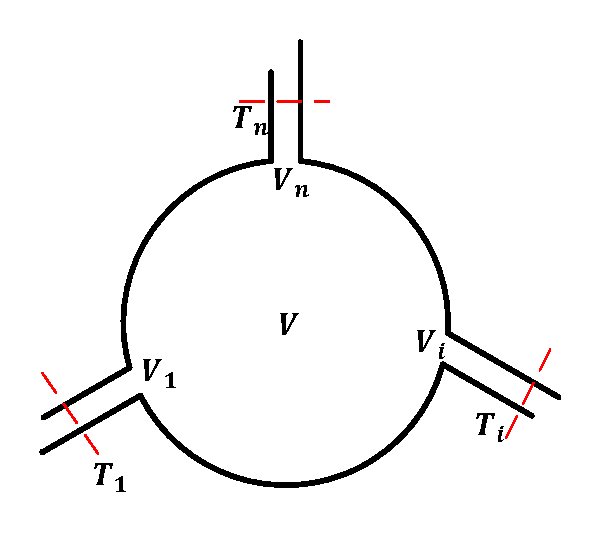
\includegraphics[width=4.5cm]{Cha5//fig5-1.pdf}
            \end{figure}
        \end{column}
    \end{columns}
\end{frame}

\begin{frame}{微波网络概念及等效关系}
    \begin{itemize}
        \item 传输线建模\\
              把传输线等效为双线,用特征参数表征。单模传输线等效为一条双线,$n$模传输线等效为n条传输线。
        \item 不连续性建模\\
              可以采用等效电路模型,也可以采用网络矩阵表征。
        \item 通过建模,射频电路等效为由传输线和不连续性网络构成的电路。射频电路就可以采用电路理论分析和设计,“场方法”转化为“路方法”。
    \end{itemize}
\end{frame}

\begin{frame}{微波网络概念及等效关系}
    当波从一传输线入射到一不连续性区域时,一部分反射会传输线,其余部分通过不连续性区域传输到其他传输线,同时在不连续性区域激发出高次模,
    这些高次模在传输线中为截止波,所以很快衰减掉。这样在不连续性附近就形成了一个能量存储区,相当于电抗元件。\\
    \hspace*{\fill}\\
    以网络的观点,不连续性区域可以看作连接传输线的网络。在传输线上适当位置选取参考面$T$,不连续性区域就可以等效为多端口网络。
    \begin{figure}
        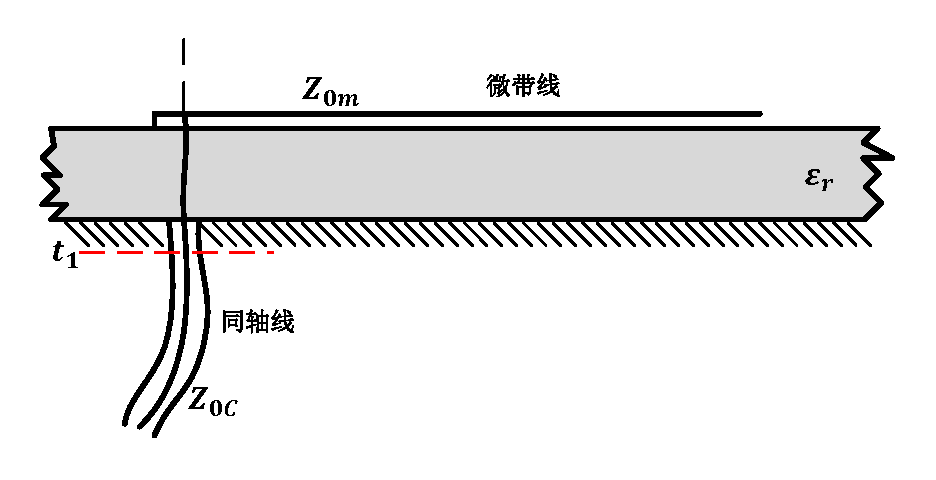
\includegraphics[width=5cm]{Cha5//fig5-2.pdf}
        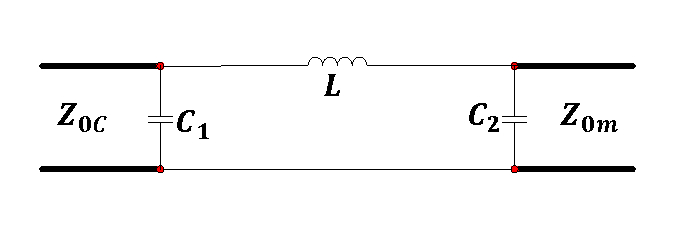
\includegraphics[width=6.5cm]{Cha5//fig5-3.pdf}
    \end{figure}
\end{frame}

\begin{frame}{微波网络概念及等效关系}
    \begin{enumerate}
        \item 微波传输线等效为双线
              \begin{itemize}
                  \item 等效阻抗:等效电压和等效电流之比
                        $$Z(z)=\frac{V(z)}{I(z)}$$
                  \item 归一化等效阻抗
                        $$z=\frac{Z(z)}{Z_0}=\frac{V(z)/\sqrt{Z_0}}{I(z)\sqrt{Z_0}}=\frac{1+\Gamma(z)}{1-\Gamma(z)}$$
                        归一化等效电压:$v(z)=V(z)/\sqrt{Z_0}$\\
                        归一化等效电流:$i(z)=I(z)\sqrt{Z_0}$
                  \item 功率\\
                        $$P=\frac{1}{2}[V(z)/\sqrt{Z_0}][I^*(z)\sqrt{Z_0}]=\frac{1}{2}v(z)i^*(z)$$
              \end{itemize}
    \end{enumerate}
\end{frame}

\begin{frame}{微波网络概念及等效关系}
    \begin{enumerate}
        \item 微波传输线等效为双线
              \begin{itemize}
                  \item 等效双线上的电压和电流可以写成入射波和反射波之和,即:
              \end{itemize}
              \begin{gather*}
                  \begin{cases}
                      V(z)=V^{+}(z)+V^{-}(z) \\
                      I(z)=I^{+}(z)-I^{-}(z)=\frac{1}{Z_0}[V^{+}(z)-V^{-}(z)]
                  \end{cases}
              \end{gather*}
              \begin{gather*}                                                                                                              \\
                  \begin{matrix*}
                      \dfrac{V(z)}{\sqrt{Z_0}}=\dfrac{V^{+}(z)}{\sqrt{Z_0}}+\dfrac{V^{-}(z)}{\sqrt{Z_0}}\\
                      I(z)\sqrt{Z_0}=\dfrac{V^{+}(z)}{\sqrt{Z_0}}-\dfrac{V^{-}(z)}{\sqrt{Z_0}}\\
                  \end{matrix*} \\
                  \quad\Downarrow\quad                                                                                                                                            \\
                  \begin{matrix*}
                      v(z)=v^{+}(z)+v^{-}(z)\\
                      i(z)=v^{+}(z)-v^{-}(z)\\
                  \end{matrix*}
              \end{gather*}
    \end{enumerate}
\end{frame}

\begin{frame}{微波网络概念及等效关系}
    \begin{enumerate}
        \item 微波传输线等效为双线
              \begin{itemize}
                  \item 归一化入射波电压模的平方正比于入射波功率,即
                        \begin{align*}
                            P^+=\frac{1}{2}|V^+(z)||I^+(z)|=\frac{|V^+(z)|^2}{2Z_0}=\frac{1}{2}\left\lvert\frac{V^+(z)}{\sqrt{Z_0}}\right\rvert^2=\frac{1}{2}|v^+(z)|^2
                        \end{align*}
                  \item 归一化反射波电压模的平方正比于反射波功率,即
                        \begin{align*}
                            P^-=\frac{1}{2}|V^-(z)||I^-(z)|=\frac{|V^-(z)|^2}{2Z_0}=\frac{1}{2}\left\lvert\frac{V^-(z)}{\sqrt{Z_0}}\right\rvert^2=\frac{1}{2}|v^-(z)|^2
                        \end{align*}
              \end{itemize}
              \saveenum
    \end{enumerate}
\end{frame}

\begin{frame}{微波网络概念及等效关系}
    \begin{enumerate}
        \resume
        \item 不均匀区等效为网络\\
              研究微波网络首先必须确定网络的参考面,参考面的位置可以任意选,但是必须考虑两点:
              \begin{itemize}
                  \item 单模传输时,参考面的位置应该尽量选取在远离不连续区域,这样参考面上的高次模场强可以忽略,只需考虑主模的场强
                  \item 选择参考面必须与传输方向相垂直,这样可使参考面上的电压和电流有着明确意义
              \end{itemize}
              网络参考面一旦确定后,所定义的微波网络就是由这些参考面所包围的区域,网络的参数也就唯一确定,如果参考面位置改变,则网络
              参数也随之改变。
    \end{enumerate}
\end{frame}

\begin{frame}{微波网络概念及等效关系}
    \begin{enumerate}
        \resume
        \item 不均匀区等效为网络
              \begin{figure}
                  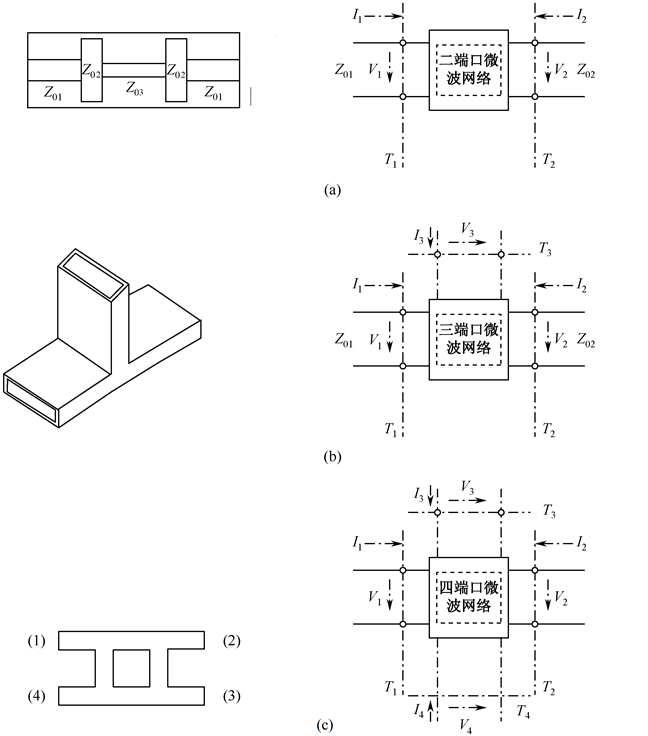
\includegraphics[width=6cm]{Cha5//fig5-4.png}
              \end{figure}
    \end{enumerate}
\end{frame}

\subsection{微波网络参量}
\begin{frame}{微波网络参量}
    \begin{enumerate}
        \item 微波网络的电路参量\\
              \begin{figure}
                  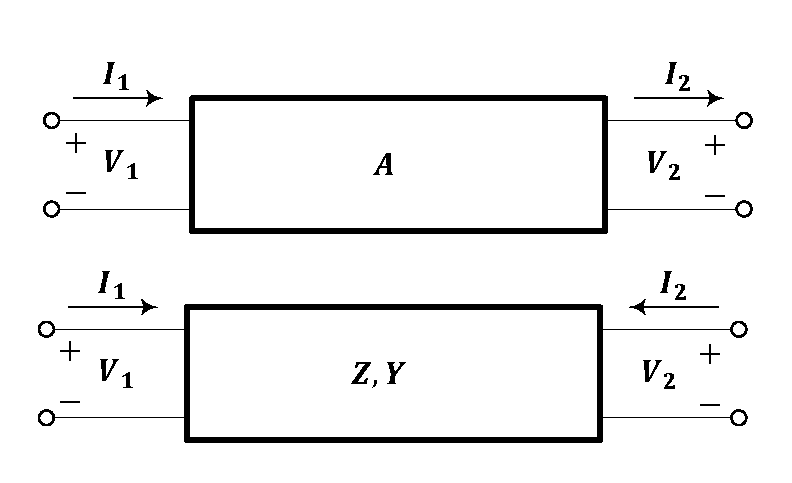
\includegraphics[width=7cm]{Cha5//fig5-5.pdf}
                  \caption{用$Z,Y和A$参数表示的二端口网络示意图}
              \end{figure}
    \end{enumerate}
\end{frame}

\begin{frame}{微波网络参量}
    \begin{enumerate}
        \item 微波网络的电路参量
              \begin{itemize}
                  \item 阻抗矩阵$[Z]$:反映电压、电流关系
              \end{itemize}
              \begin{figure}
                  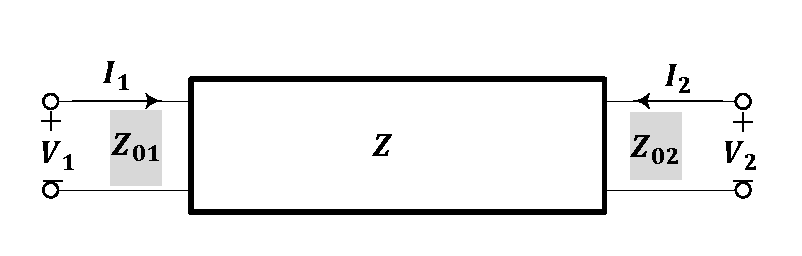
\includegraphics[width=7cm]{Cha5//fig5-6.pdf}
              \end{figure}
              \begin{gather}
                  \begin{bmatrix*}
                      V_1\\
                      V_2\\
                  \end{bmatrix*}
                  =
                  \begin{bmatrix*}
                      Z_{11} & Z_{12}\\
                      Z_{21} & Z_{22}\\
                  \end{bmatrix*}
                  \begin{bmatrix*}
                      I_1 \\
                      I_2 \\
                  \end{bmatrix*}\label{eqn5-1}\\
                  [V]=[Z][I]\label{eqn5-2}
              \end{gather}
    \end{enumerate}
\end{frame}

\begin{frame}{微波网络参量}
    \begin{enumerate}
        \item 微波网络的电路参量
              \begin{itemize}
                  \item 网络的“开路”参数:“自阻抗”和“转移阻抗”
              \end{itemize}
              \begin{gather*}
                  \begin{bmatrix*}
                      V_1\\
                      V_2\\
                  \end{bmatrix*}
                  =
                  \begin{bmatrix*}
                      Z_{11} & Z_{12}\\
                      Z_{21} & Z_{22}\\
                  \end{bmatrix*}
                  \begin{bmatrix*}
                      I_1 \\
                      I_2 \\
                  \end{bmatrix*}\\
                  \begin{matrix*}
                      V_1=Z_{11}\cdot I_1+Z_{12}\cdot I_2\\
                      V_2=Z_{21}\cdot I_1+Z_{22}\cdot I_2\\
                  \end{matrix*}
                  \qquad Z=\frac{V}{I}\\
                  \begin{matrix*}
                      Z_{11}=\dfrac{V_1}{I_1}\bigg|_{I_2=0} & Z_{21}=\dfrac{V_2}{I_1}\bigg|_{I_2=0} & 2端口开路 \\
                      Z_{22}=\dfrac{V_2}{I_2}\bigg|_{I_1=0} & Z_{12}=\dfrac{V_1}{I_2}\bigg|_{I_1=0} & 1端口开路 \\
                  \end{matrix*}
              \end{gather*}
    \end{enumerate}
\end{frame}

\begin{frame}{微波网络参量}
    \begin{enumerate}
        \item 微波网络的电路参量
              \begin{itemize}
                  \item 归一化阻抗矩阵$[z]$:用$Z_{01},Z_{02}$归一化
              \end{itemize}
              \begin{gather}
                  \begin{bmatrix*}
                      v_1\\
                      v_2\\
                  \end{bmatrix*}
                  =
                  \begin{bmatrix*}
                      \frac{1}{\sqrt{Z_{01}}} & 0\\
                      0 & \frac{1}{\sqrt{Z_{02}}}\\
                  \end{bmatrix*}
                  \begin{bmatrix*}
                      V_1 \\
                      V_2 \\
                  \end{bmatrix*}\label{eqn5-3}\\
                  \hspace*{\fill}
                  \begin{bmatrix*}
                      i_1\\
                      i_2\\
                  \end{bmatrix*}
                  =
                  \begin{bmatrix*}
                      \sqrt{Z_{01}} & 0\\
                      0 & \sqrt{Z_{02}}\\
                  \end{bmatrix*}
                  \begin{bmatrix*}
                      I_1 \\
                      I_2 \\
                  \end{bmatrix*}
                  \label{eqn5-4}
              \end{gather}
              根据式(\ref{eqn5-1})和式(\ref{eqn5-3}),(\ref{eqn5-4})有
              \begin{gather*}
                  \begin{bmatrix*}
                      \frac{1}{\sqrt{Z_{01}}} & 0\\
                      0 & \frac{1}{\sqrt{Z_{02}}}\\
                  \end{bmatrix*}^{-1}
                  \begin{bmatrix*}
                      v_1 \\
                      v_2 \\
                  \end{bmatrix*}
                  =
                  \begin{bmatrix*}
                      Z_{11} & Z_{12}\\
                      Z_{21} & Z_{22}\\
                  \end{bmatrix*}
                  \begin{bmatrix*}
                      \sqrt{Z_{01}} & 0\\
                      0 & \sqrt{Z_{02}}\\
                  \end{bmatrix*}^{-1}
                  \begin{bmatrix*}
                      i_1\\
                      i_2\\
                  \end{bmatrix*}
              \end{gather*}
    \end{enumerate}
\end{frame}

\begin{frame}{微波网络参量}
    \begin{enumerate}
        \item 微波网络的电路参量
              \begin{itemize}
                  \item 归一化阻抗矩阵$[z]$:用$Z_{01},Z_{02}$归一化
              \end{itemize}
              \begin{gather}
                  \begin{bmatrix*}
                      v_1 \\
                      v_2 \\
                  \end{bmatrix*}
                  =
                  \begin{bmatrix*}
                      \frac{1}{\sqrt{Z_{01}}} & 0\\
                      0 & \frac{1}{\sqrt{Z_{02}}}\\
                  \end{bmatrix*}
                  \begin{bmatrix*}
                      Z_{11} & Z_{12}\\
                      Z_{21} & Z_{22}\\
                  \end{bmatrix*}
                  \begin{bmatrix*}
                      \sqrt{Z_{01}} & 0\\
                      0 & \sqrt{Z_{02}}\\
                  \end{bmatrix*}^{-1}
                  \begin{bmatrix*}
                      i_1\\
                      i_2\\
                  \end{bmatrix*}\label{eqn5-5}\\
                  \Rightarrow
                  \begin{bmatrix*}
                      v_1 \\
                      v_2 \\
                  \end{bmatrix*}
                  =
                  \begin{bmatrix*}
                      \dfrac{Z_{11}}{Z_{01}} & \dfrac{Z_{12}}{\sqrt{Z_{01}\cdot Z_{02}}}\\
                      \dfrac{Z_{21}}{\sqrt{Z_{01}\cdot Z_{02}}} & \dfrac{Z_{22}}{Z_{02}}\\
                  \end{bmatrix*}
                  \begin{bmatrix*}
                      i_1 \\
                      i_2 \\
                  \end{bmatrix*}\label{eqn5-6}
                  \qquad
                  [v]=[z][i]
              \end{gather}
    \end{enumerate}
\end{frame}

\begin{frame}{微波网络参量}
    \begin{enumerate}
        \item 微波网络的电路参量
              \begin{table}
                  \caption{阻抗矩阵单元物理意义}
                  \footnotesize
                  \begin{tabular}{|c|c|c|}
                      \hline
                      \textbf{阻抗矩阵阵元} & \textbf{计算公式}                        & \textbf{物理意义}    \\ \hline
                      $Z_{11}$        & $\dfrac{V_1}{I_1}\bigg\vert_{I_2=0}$ & 输出端口开路情况下的输入阻抗   \\ \hline
                      $Z_{12}$        & $\dfrac{V_1}{I_2}\bigg\vert_{I_1=0}$ & 输入端口开路情况下的反向传输阻抗 \\ \hline
                      $Z_{21}$        & $\dfrac{V_2}{I_1}\bigg\vert_{I_2=0}$ & 输出端口开路情况下的正向传输阻抗 \\ \hline
                      $Z_{22}$        & $\dfrac{V_2}{I_2}\bigg\vert_{I_1=0}$ & 输入端口开路情况下的输出阻抗   \\ \hline
                  \end{tabular}
              \end{table}
    \end{enumerate}
\end{frame}

\begin{frame}{微波网络参量}
    \begin{enumerate}
        \item 微波网络的电路参量
              \begin{itemize}
                  \item 导纳矩阵$[Y]$
                        \begin{figure}
                            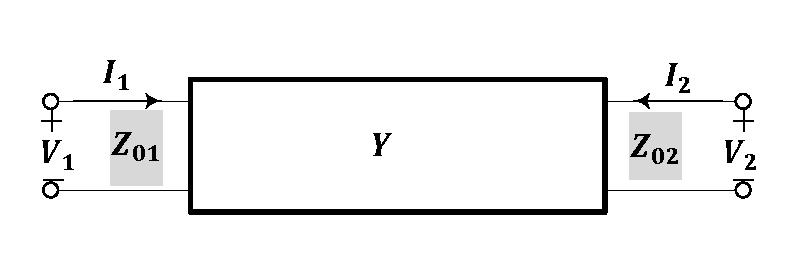
\includegraphics[width=8cm]{Cha5//fig5-7.pdf}
                        \end{figure}
                        \begin{gather*}
                            \begin{bmatrix*}
                                I_1\\
                                I_2\\
                            \end{bmatrix*}
                            =
                            \begin{bmatrix*}
                                Y_{11} & Y_{12}\\
                                Y_{21} & Y_{22}\\
                            \end{bmatrix*}
                            \begin{bmatrix*}
                                V_1 \\
                                V_2 \\
                            \end{bmatrix*}\\
                            [I]=[Y][V]
                        \end{gather*}
              \end{itemize}
    \end{enumerate}
\end{frame}

\begin{frame}{微波网络参量}
    \begin{enumerate}
        \item 微波网络的电路参量
              \begin{itemize}
                  \item 网络的“短路”参数:“自导纳”和“转移导纳”
                        \begin{gather*}
                            \begin{bmatrix*}
                                I_1\\
                                I_2\\
                            \end{bmatrix*}
                            =
                            \begin{bmatrix*}
                                Y_{11} & Y_{12}\\
                                Y_{21} & Y_{22}\\
                            \end{bmatrix*}
                            \begin{bmatrix*}
                                V_1 \\
                                V_2 \\
                            \end{bmatrix*}\\
                            Y_{ij}=\frac{I_i}{V_j}\bigg|_{V_k=0,k\neq j}
                        \end{gather*}
                        所有其他端口短路时,驱动端口$j$的电压为$V_j$时在端口$i$测得的短路电流来确定。
                        \begin{gather*}
                            [i]=[y][v] \qquad
                            [y]=
                            \begin{bmatrix*}
                                Y_{11}Z_{01} & Y_{12}\sqrt{Z_{01}Z_{02}} \\
                                Y_{21}\sqrt{Z_{01}Z_{02}} & Y_{22}Z_{02} \\
                            \end{bmatrix*}
                        \end{gather*}
              \end{itemize}
    \end{enumerate}
\end{frame}

\begin{frame}{微波网络参量}
    \begin{enumerate}
        \item 微波网络的电路参量
              \begin{table}
                  \caption{导纳矩阵单元物理意义}
                  \footnotesize
                  \begin{tabular}{|c|c|c|}
                      \hline
                      \textbf{导纳矩阵阵元} & \textbf{计算公式}                        & \textbf{物理意义}     \\ \hline
                      $Y_{11}$        & $\dfrac{I_1}{V_1}\bigg\vert_{V_2=0}$ & 输出端口短路情况下的输入导纳    \\ \hline
                      $Y_{12}$        & $\dfrac{I_1}{V_2}\bigg\vert_{V_1=0}$ & 输入端口短路路情况下的反向传输导纳 \\ \hline
                      $Y_{21}$        & $\dfrac{I_2}{V_1}\bigg\vert_{V_2=0}$ & 输出端口短路情况下的正向传输导纳  \\ \hline
                      $Y_{22}$        & $\dfrac{I_2}{V_2}\bigg\vert_{V_1=0}$ & 输入端口短路情况下的输出导纳    \\ \hline
                  \end{tabular}
              \end{table}
    \end{enumerate}
\end{frame}

\begin{frame}{微波网络参量}
    \begin{enumerate}
        \item 微波网络的电路参量
              \begin{itemize}
                  \item 转移矩阵$[A]$
                        \begin{figure}
                            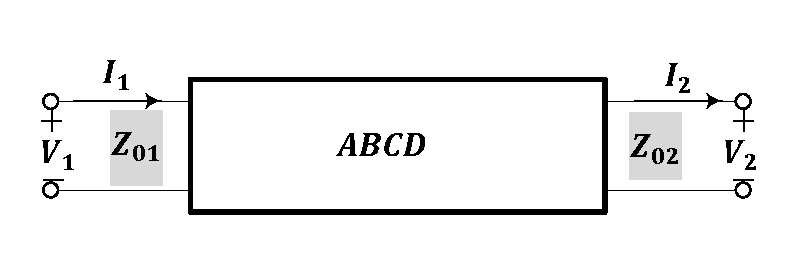
\includegraphics[width=8cm]{Cha5//fig5-8.pdf}
                        \end{figure}
                        \begin{gather*}
                            \begin{bmatrix*}
                                V_1 \\
                                I_1 \\
                            \end{bmatrix*}
                            =
                            \begin{bmatrix*}
                                A & B \\
                                C & D \\
                            \end{bmatrix*}
                            \begin{bmatrix*}
                                V_2 \\
                                I_2 \\
                            \end{bmatrix*}\quad\rightarrow\quad
                            \begin{cases}
                                V_1=A\cdot V_2+B\cdot I_2 \\
                                I_1=C\cdot V_2+D\cdot I_2
                            \end{cases}\\
                            A=\frac{V_1}{V_2}\bigg|_{I_2=0}\qquad C=\frac{I_1}{V_2}\bigg|_{I_2=0}\qquad 2端口开路\\
                            B+\frac{V_1}{I_2}\bigg|_{V_2=0}\qquad D=\frac{I_1}{I_2}\bigg|_{V_2=0}\qquad 2端口短路
                        \end{gather*}
              \end{itemize}
    \end{enumerate}
\end{frame}

\begin{frame}{微波网络参量}
    \begin{enumerate}
        \item 微波网络的电路参量
              \begin{table}
                  \caption{导纳矩阵单元物理意义}
                  \footnotesize
                  \begin{tabular}{|c|c|c|}
                      \hline
                      \textbf{导纳矩阵阵元} & \textbf{计算公式}                        & \textbf{物理意义}    \\ \hline
                      $A$             & $\dfrac{V_1}{V_2}\bigg\vert_{I_2=0}$ & 输出端口开路情况下的反向电压增益 \\ \hline
                      $B$             & $\dfrac{V_1}{I_2}\bigg\vert_{V_2=0}$ & 输出端口短路路情况下的互阻抗   \\ \hline
                      $C$             & $\dfrac{I_1}{V_2}\bigg\vert_{I_2=0}$ & 输出端口开路情况下的互导纳    \\ \hline
                      $D$             & $\dfrac{I_1}{I_2}\bigg\vert_{V_2=0}$ & 输出端口短路情况下的反向电流增益 \\ \hline
                  \end{tabular}
              \end{table}
    \end{enumerate}
\end{frame}

\begin{frame}{微波网络参量}
    \begin{enumerate}
        \item 微波网络的电路参量
              \begin{itemize}
                  \item 归一化转移矩阵$[a]$
              \end{itemize}
              \begin{gather*}
                  \begin{bmatrix*}
                      v_1 \\
                      i_1 \\
                  \end{bmatrix*}
                  =[a]
                  \begin{bmatrix*}
                      v_2 \\
                      i_2 \\
                  \end{bmatrix*}
                  \qquad
                  [a]=
                  \begin{bmatrix*}
                      A\sqrt{\dfrac{Z_{02}}{Z_{01}}} & \dfrac{B}{\sqrt{Z_{01}Z_{02}}} \\
                      C\sqrt{Z_{01}Z_{02}} & D\sqrt{\dfrac{Z_{01}}{Z_{02}}} \\
                  \end{bmatrix*}
              \end{gather*}
    \end{enumerate}
\end{frame}

\begin{frame}{微波网络参量}
    \begin{enumerate}
        \item 微波网络的电路参量
              \begin{itemize}
                  \item 转移矩阵$[A]$的用途——网络的级联(Cascade)
              \end{itemize}
              \begin{figure}
                  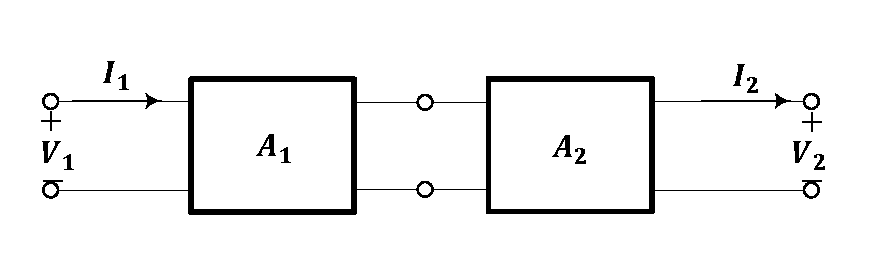
\includegraphics[width=10cm]{Cha5//fig5-9.pdf}
              \end{figure}
              \begin{gather*}
                  \begin{bmatrix*}
                      V_1 \\
                      I_1 \\
                  \end{bmatrix*}=
                  \begin{bmatrix*}
                      A & B \\
                      C & D \\
                  \end{bmatrix*}
                  \begin{bmatrix*}
                      V_2 \\
                      I_2
                  \end{bmatrix*}\\
                  \begin{bmatrix*}
                      A & B \\
                      C & D \\
                  \end{bmatrix*}=
                  \begin{bmatrix*}
                      A_1 & B_1 \\
                      C_1 & D_1 \\
                  \end{bmatrix*}
                  \begin{bmatrix*}
                      A_2 & B_2 \\
                      C_2 & D_2 \\
                  \end{bmatrix*}
              \end{gather*}
    \end{enumerate}
\end{frame}

\begin{frame}{微波网络参量}
    \begin{enumerate}
        \item 微波网络的电路参量
              \begin{itemize}
                  \item 小结:“电路”参量——反映电压、电流关系
              \end{itemize}
              \begin{gather*}
                  [V]={\color{red}{[Z]}}[I] \qquad [v]={\color{red}{[z]}}[i] \\
                  [I]={\color{red}{[Y]}}[V] \qquad [i]={\color{red}{[y]}}[v] \\
                  \begin{bmatrix*}
                      V_1 \\
                      I_1 \\
                  \end{bmatrix*}={\color{red}{[A]}}
                  \begin{bmatrix*}
                      V_2 \\
                      I_2 \\
                  \end{bmatrix*} \qquad
                  \begin{bmatrix*}
                      v_1 \\
                      i_1 \\
                  \end{bmatrix*}={\color{red}{[a]}}
                  \begin{bmatrix*}
                      v_2 \\
                      i_2 \\
                  \end{bmatrix*}
              \end{gather*}
              \saveenum
    \end{enumerate}
\end{frame}

\begin{frame}{微波网络参量}
    \begin{enumerate}
        \resume
        \item 微波网络的波参量\\
              反映端口的入射波和反射波之间的关系。\\
              \begin{itemize}
                  \item 散射参量——$[S]$
                  \item 传输参量——$[T]$
              \end{itemize}
              \begin{figure}
                  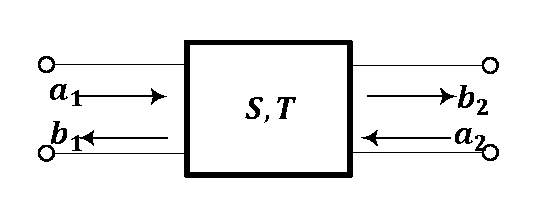
\includegraphics[width=8cm]{Cha5//fig5-10.pdf}
              \end{figure}
              \begin{itemize}
                  \item $a$:归一化入射波场强复振幅
                  \item $b$:归一化反射波场强复振幅
              \end{itemize}
    \end{enumerate}
\end{frame}

\begin{frame}{微波网络参量}
    \begin{enumerate}
        \resume
        \item 微波网络的波参量\\
              由传输线理论已经导出
              \begin{gather*}
                  \begin{cases}
                      V=V_0^+\mathrm{e}^{-\gamma z}+V_0^-\mathrm{e}^{\gamma z} \\
                      I=\dfrac{1}{Z_0}(V_0^+\mathrm{e}^{-\gamma z}-V_0^-\mathrm{e}^{\gamma z})
                  \end{cases}
              \end{gather*}
              用入射波和反射波表示,其中
              \begin{gather*}
                  \begin{cases}
                      V_0^+\mathrm{e}^{-\gamma z}=\dfrac{1}{2}(V+IZ_0) \\
                      V_0^-\mathrm{e}^{+\gamma z}=\dfrac{1}{2}(V-IZ_0)
                  \end{cases}
              \end{gather*}
    \end{enumerate}
\end{frame}

\begin{frame}{微波网络参量}
    \begin{enumerate}
        \resume
        \item 微波网络的波参量
              \begin{itemize}
                  \item $S$散射参数\\
                        首先定义出入射波和散射波($a$和$b$)。其中,散射波是广义的(理论上可以是任意方向)反射波。
              \end{itemize}
              \begin{gather*}
                  \begin{cases}
                      a=\dfrac{V_0^+\mathrm{e}^{-\gamma z}}{\sqrt{Z_0}}=\dfrac{1}{2}\left(\dfrac{V}{\sqrt{Z_0}}+I\sqrt{Z_0}\right) \\
                      b=\dfrac{V_0^-\mathrm{e}^{+\gamma z}}{\sqrt{Z_0}}=\dfrac{1}{2}\left(\dfrac{V}{\sqrt{Z_0}}-I\sqrt{Z_0}\right)
                  \end{cases}\\
                  a=\dfrac{1}{2}(v+i),b=\dfrac{1}{2}(v-i)\qquad
                  \begin{cases}
                      v=a+b \\
                      i=a-b
                  \end{cases}
              \end{gather*}
    \end{enumerate}
\end{frame}

\begin{frame}{微波网络参量}
    \begin{enumerate}
        \resume
        \item 微波网络的波参量\\
              \begin{itemize}
                  \item 散射参量——归一化散射矩阵
              \end{itemize}
              \begin{figure}
                  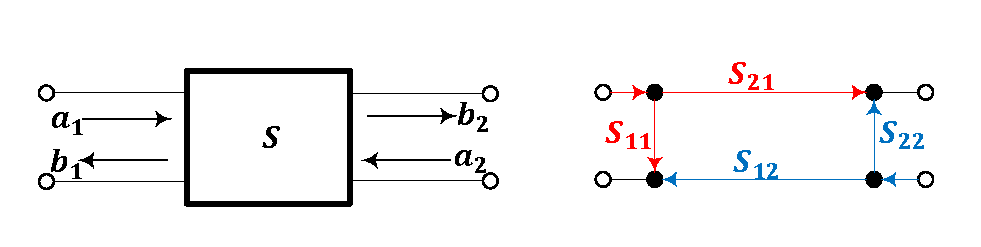
\includegraphics[width=10cm]{Cha5//fig5-11.pdf}
              \end{figure}
              \begin{gather*}
                  \begin{bmatrix*}
                      b_1 \\
                      b_2 \\
                  \end{bmatrix*}=
                  \begin{bmatrix*}
                      S_{11} & S_{12} \\
                      S_{21} & S_{22} \\
                  \end{bmatrix*}
                  \begin{bmatrix*}
                      a_1 \\
                      a_2 \\
                  \end{bmatrix*}\\
                  \begin{cases}
                      b_1=S_{11}\cdot a_1+S_{12}\cdot a_2 \\
                      b_2=S_{21}\cdot a_1+S_{22}\cdot a_2
                  \end{cases}
              \end{gather*}
    \end{enumerate}
\end{frame}

\begin{frame}{微波网络参量}
    \begin{enumerate}
        \resume
        \item 微波网络的波参量\\
              \begin{gather*}
                  \begin{matrix*}
                      S_{11}=\dfrac{b_1}{a_1}\bigg|_{a_2=0} & S_{21}=\dfrac{b_2}{a_1}\bigg|_{a_2=0} & \text{\footnotesize{2端口匹配}} \\
                      \text{\footnotesize{表示端口2接匹配负载时,}}  & \text{\footnotesize{端口1到端口2的传输系数}} & \\
                      \text{\footnotesize{端口1的反射系数}}  &  &  \\
                      S_{22}=\dfrac{b_2}{a_2}\bigg|_{a_1=0} & S_{12}=\dfrac{b_1}{a_2}\bigg|_{a_1=0} & \text{\footnotesize{1端口匹配}} \\
                      \text{\footnotesize{表示端口1接匹配负载时,}}  & \text{\footnotesize{端口2到端口1的传输系数}} & \\
                      \text{\footnotesize{端口2的反射系数}}  &  &  \\
                  \end{matrix*}
              \end{gather*}
    \end{enumerate}
\end{frame}

\begin{frame}{微波网络参量}
    \begin{enumerate}
        \resume
        \item 微波网络的波参量\\
              \begin{itemize}
                  \item 传输参量——传输矩阵
              \end{itemize}
              \begin{figure}
                  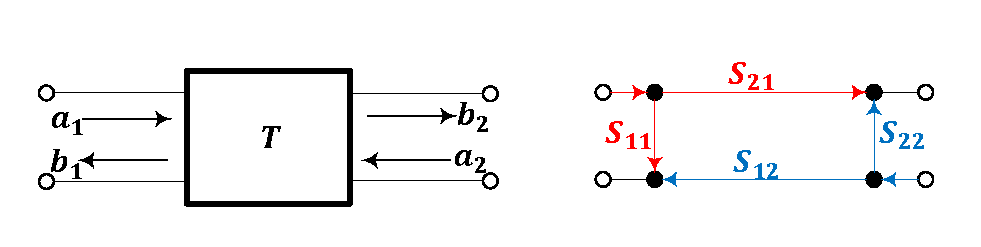
\includegraphics[width=10cm]{Cha5//fig5-12.pdf}
              \end{figure}
              \begin{gather*}
                  \begin{bmatrix*}
                      a_1 \\
                      b_1 \\
                  \end{bmatrix*}=
                  \begin{bmatrix*}
                      T_{11} & T_{12} \\
                      T_{21} & T_{22} \\
                  \end{bmatrix*}
                  \begin{bmatrix*}
                      b_2 \\
                      a_2 \\
                  \end{bmatrix*}\\
                  \begin{cases}
                      a_1 = T_{11}\cdot b_2 + T_{12}\cdot a_2 \\
                      b_1 = T_{21}\cdot b_2 + T_{22}\cdot a_2
                  \end{cases}
                  T_{11} = \dfrac{1}{\left(\dfrac{b_2}{a_1}\bigg|_{a_2=0}\right)}
              \end{gather*}
              $T_{11}$物理含义:端口2匹配情况下,端口1到端口2的“传输系数”的倒数。
    \end{enumerate}
\end{frame}

\begin{frame}{微波网络参量}
    \begin{enumerate}
        \resume
        \item 微波网络的波参量\\
              \begin{itemize}
                  \item $n$端口网络
              \end{itemize}
              \begin{figure}
                  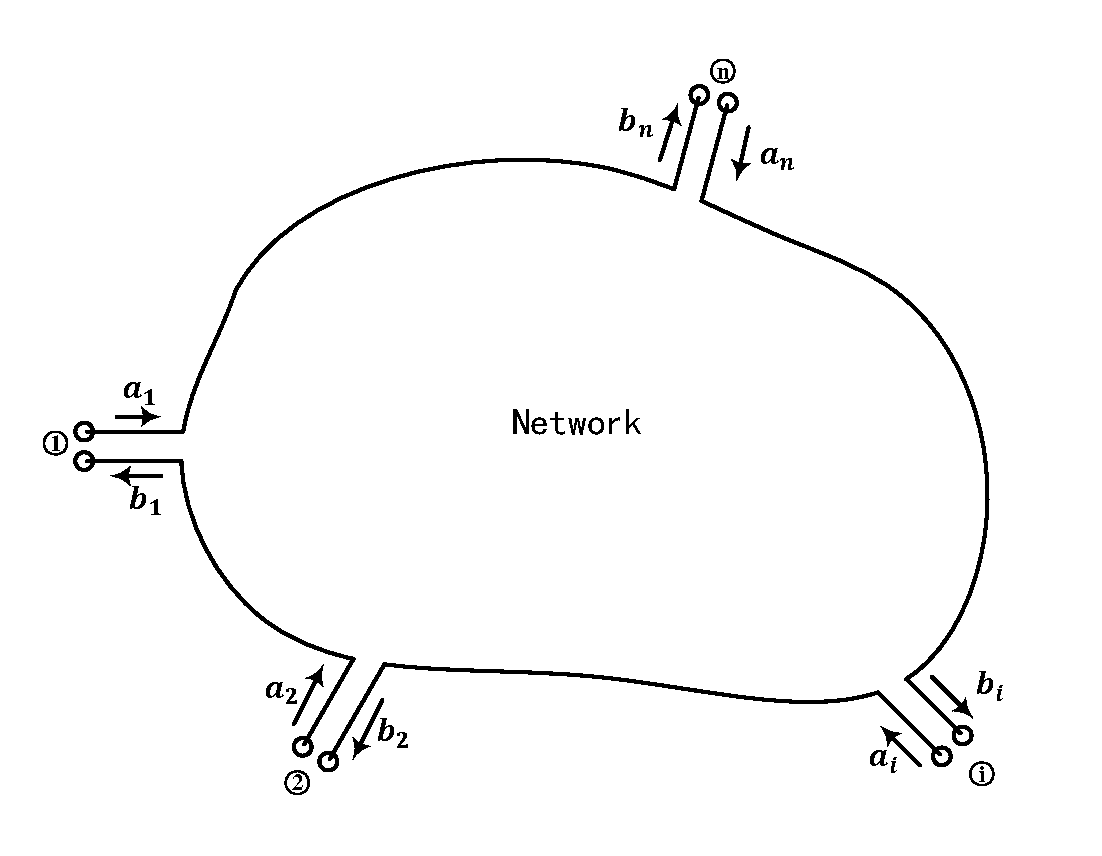
\includegraphics[width=8cm]{Cha5//fig5-13.pdf}
              \end{figure}
    \end{enumerate}
\end{frame}

\begin{frame}{微波网络参量}
    \begin{enumerate}
        \resume
        \item 微波网络的波参量 \\
              \begin{itemize}
                  \item $N$端口网络
              \end{itemize}
              \begin{gather*}
                  \begin{bmatrix*}
                      b_1 \\
                      b_2 \\
                      \vdots \\
                      b_n
                  \end{bmatrix*}=
                  \begin{bmatrix*}
                      S_{11} & S_{12} & \cdots & S_{1n} \\
                      S_{21} & S_{22} & \cdots & S_{2n} \\
                      \vdots & \vdots & \vdots & \vdots \\
                      S_{n1} & S_{n2} & \cdots & S_{nn} \\
                  \end{bmatrix*}
                  \begin{bmatrix*}
                      a_1 \\
                      a_2 \\
                      \vdots \\
                      a_n
                  \end{bmatrix*}
              \end{gather*}
              \begin{align*}
                   & \begin{matrix*}
                         S_{ii}=\dfrac{b_i}{a_i}\bigg|_{a_k=0} & (i,k=1,2,3,\cdots,n; k\neq i) \\
                     \end{matrix*}           \\
                   & \text{\scriptsize{\color{blue}{表示除端口i之外其余各个端口均接匹配负载时端口i的反射系数}}}                 \\
                   & \begin{matrix*}
                         S_{ji}=\dfrac{b_j}{a_i}\bigg|_{a_k=0} & (i,j,k=1,2,3,\cdots,n; j\neq i,k\neq i) \\
                     \end{matrix*} \\
                   & \text{\scriptsize{\color{blue}{表示除端口i之外其余各个端口均接匹配负载时端口i到端口j的传输系数}}}
              \end{align*}
              \saveenum
    \end{enumerate}
\end{frame}

\begin{frame}{微波网络参量}
    [例1]\quad 在特性阻抗为$Z_0$的传输线上串接阻抗$z$(归一化$z$),求该串接阻抗的散射参数。\\
    \begin{columns}
        \begin{column}{0.5\linewidth}
            解:令端口2接匹配负载,归一化后为1,则$a_2=0$,有
            \begin{gather*}
                \begin{cases}
                    i_1=\dfrac{v_1}{z+1} \\
                    i_1=-i_2
                \end{cases}\\
                因为
                \begin{cases}
                    a_1-b_1=\dfrac{v_1}{z+1}=\dfrac{a_1+b_1}{z+1} \\
                    a_1-b_1=b_2
                \end{cases}
            \end{gather*}
        \end{column}
        \begin{column}{0.5\linewidth}
            \begin{figure}
                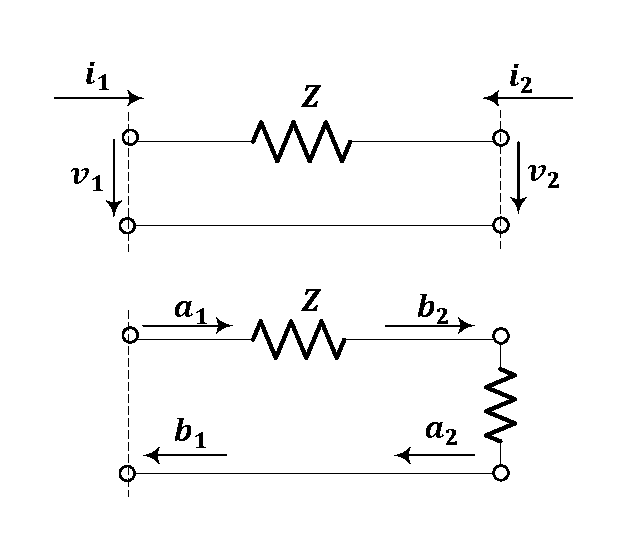
\includegraphics[width=6cm]{Cha5//fig5-14.pdf}
            \end{figure}
        \end{column}
    \end{columns}
\end{frame}

\begin{frame}{微波网络参量}
    \begin{align*}
         & b_1=\dfrac{z}{z+2}a_1,b_2=\dfrac{2}{z+2}a_1                 \\
         & S_{11}=\dfrac{b_1}{a_1}\bigg|_{a_2=0}=\dfrac{z}{z+2} \qquad
        S_{21}=\dfrac{b_2}{a_1}\bigg|_{a_2=0}=\dfrac{2}{z+2}
    \end{align*}
    同理,设端口1接匹配负载,类似得:
    \begin{align*}
        S_{22}=\dfrac{b_2}{a_2}\bigg|_{a_1=0}=\dfrac{z}{z+2} \qquad S_{12}=\dfrac{b_1}{a_2}\bigg|_{a_1=0}=\dfrac{2}{z+2}
    \end{align*}
    \begin{gather*}
        [S]=
        \begin{bmatrix*}
            \dfrac{z}{2+z} & \dfrac{2}{2+z} \\
            \dfrac{2}{2+z} & \dfrac{z}{2+z} \\
        \end{bmatrix*}
    \end{gather*}
\end{frame}

\begin{frame}{微波网络参量}
    [例2] \quad 在特性阻抗为$Z_0$的传输线上并联导纳$Y$(归一化$y$),求该并联导纳的散射参数。
    \begin{columns}
        \begin{column}{0.5\linewidth}
            解:令端口2接匹配负载,归一化后为1,则$a_2=0$,有
            \begin{gather*}
                \begin{cases}
                    i_1=v_1(y+1) \\
                    v_1=v_2
                \end{cases}
                \\
                \begin{cases}
                    a_1-b_1=(a_1+b_1)(y+1) \\
                    a_1+b_1=a_2+b_2
                \end{cases}
            \end{gather*}
        \end{column}
        \begin{column}{0.5\linewidth}
            \begin{figure}
                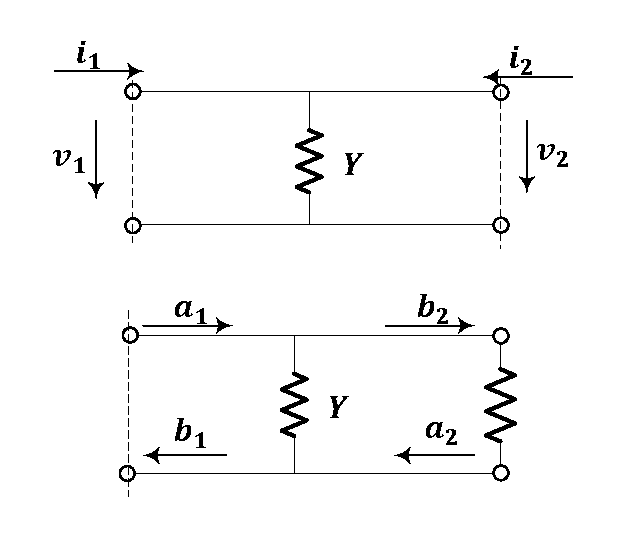
\includegraphics[width=6cm]{Cha5//fig5-15.pdf}
            \end{figure}
        \end{column}
    \end{columns}
\end{frame}

\begin{frame}{微波网络参量}
    \begin{gather*}
        \begin{cases}
            a_1 y=-b_1(y+2) \\
            \dfrac{2}{y+2}a_2=b_2
        \end{cases}
    \end{gather*}
    \begin{gather*}
        S_{11}=\dfrac{b_1}{a_1}\bigg|_{a_2=0}=-\dfrac{y}{y+2}\quad
        S_{21}=\dfrac{b_2}{a_1}\bigg|_{a_2=0}=\dfrac{2}{y+2}
    \end{gather*}
    同理,设端口1接匹配负载,类似得:

    \begin{gather*}
        S_{22}=\dfrac{b_2}{a_2}\bigg|_{a_1=0}=-\dfrac{y}{y+2}\quad
        S_{12}=\dfrac{b_1}{a_2}\bigg|_{a_1=0}=\dfrac{2}{y+2}\\
        [S]=
        \begin{bmatrix*}
            \dfrac{-y}{2+y} & \dfrac{2}{2+y} \\
            \dfrac{2}{2+y} & \dfrac{-y}{2+y} \\
        \end{bmatrix*}
    \end{gather*}
\end{frame}

\begin{frame}{微波网络参量}
    [例3]\quad 已知二端口网络的散射矩阵$[S]$,端口2接有负载$Z_L$,反射系数为$\Gamma_L$,求网络端口1的反射系数以及输入阻抗。
    \begin{figure}
        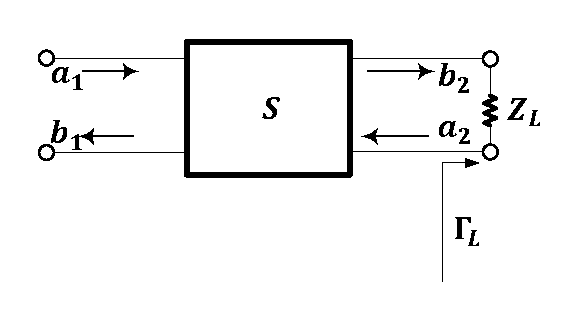
\includegraphics[width=8cm]{Cha5//fig5-16.pdf}
    \end{figure}
\end{frame}

\begin{frame}{微波网络参量}
    网络的散射参量矩阵
    \begin{gather*}
        \begin{bmatrix*}
            b_1 \\
            b_2 \\
        \end{bmatrix*}
        =
        \begin{bmatrix*}
            S_{11} & S_{12} \\
            S_{21} & S_{22} \\
        \end{bmatrix*}
        \begin{bmatrix*}
            a_1 \\
            a_2 \\
        \end{bmatrix*}\\
        \begin{cases}
            b_1=S_{11}\cdot a_1+S_{12}\cdot a_2 \\
            b_2=S_{21}\cdot a_1+S_{22}\cdot a_2
        \end{cases}
    \end{gather*}
    根据$\Gamma_L=\dfrac{a_2}{b_2}$可得
    \begin{gather*}
        \begin{cases}
            b_1=S_{11}\cdot a_1+S_{12}\cdot a_2 \\
            1=S_{21}\dfrac{a_1}{b_2}+S_{22}\dfrac{a_2}{b_2}=S_{21}\dfrac{a_1}{b_2}+S_{22}\Gamma_L
        \end{cases}
    \end{gather*}
    得
    \begin{gather*}
        b_2=\frac{S_{21}a_1}{1-S_{22}\Gamma_L}\\
        a_2=\Gamma_L \cdot b_2=\dfrac{S_{21}\Gamma_L a_1}{1-S_{22}\Gamma_L}
    \end{gather*}
\end{frame}

\begin{frame}{微波网络参量}
    \begin{align*}
        b_1=S_{11}a_1+\dfrac{S_{12}S_{21}\Gamma_L}{1-S_{22}\Gamma_L}a_1
    \end{align*}
    端口1的反射系数:
    $$\Gamma_{in}=\frac{b_1}{a_1}\Rightarrow \Gamma_{in}=S_{11}+\frac{S_{12}S_{21}\Gamma_L}{1-S_{22}\Gamma_L}$$
    端口1的阻抗:
    $$Z_{in}=\frac{1+\Gamma_{in}}{1-\Gamma_{in}}Z_0$$
    \begin{itemize}
        \item 网络自身的$S$参量以及因负载的反射透过网络在端口1造成的影响
        \item 在微波测量中非常重要
    \end{itemize}
\end{frame}

\begin{frame}{微波网络参量}
    [例4]\quad 一段均匀、无耗微波传输线,特性阻抗$Z_0$,电长度$\theta$,求$S$矩阵
    \begin{figure}
        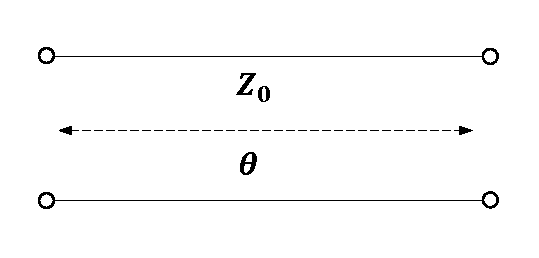
\includegraphics[width=7cm]{Cha5//fig5-17.pdf}
    \end{figure}
    解:对于无耗均匀传输线,端口1的电压波$V_1^+(a_1)$推进到端口2为$V_2^-(b_2)$,$V_1^+(a_1)$比$V_2^-(b_2)$超前相角$\theta$,则有关系式
    \begin{align*}
        a_1=b_2\mathrm{e}^{\mathrm{j}\theta}\quad b_1=0
    \end{align*}
    \begin{itemize}
        \item 令端口2接匹配负载,归一化后为1
        \item $a_2=0$
    \end{itemize}
\end{frame}

\begin{frame}{微波网络参量}
    同理,端口2的电压波$V_2^+(a_2)$推进到端口1为$V_1^-(b_1)$,$V_2^+(a_2)$比$V_1^-(b_1)$超前相角$\theta$,则有关系式
    \begin{align*}
        a_2=b_1\mathrm{e}^{\mathrm{j}\theta}\quad b_2=0
    \end{align*}
    \begin{itemize}
        \item 令端口1接匹配负载,归一化后为1
        \item $a_1=0$
    \end{itemize}
    \begin{align*}
        S_{11}=\frac{b_1}{a_1}\bigg|_{a_2=0}=\frac{0}{b_2\mathrm{e}^{\mathrm{j}\theta}}=0\qquad
        S_{12}=\frac{b_1}{a_2}\bigg|_{a_1=0}=\frac{b_1}{b_1\mathrm{e}^{\mathrm{j}\theta}}=\mathrm{e}^{-\mathrm{j}\theta} \\
        S_{22}=\frac{b_2}{a_2}\bigg|_{a_1=0}=\frac{0}{b_1\mathrm{e}^{\mathrm{j}\theta}}=0\qquad
        S_{21}=\frac{b_2}{a_1}\bigg|_{a_2=0}=\frac{b_2}{b_2\mathrm{e}^{\mathrm{j}\theta}}=\mathrm{e}^{-\mathrm{j}\theta}
    \end{align*}
\end{frame}

\begin{frame}{微波网络参量}
    \begin{enumerate}
        \resume
        \item 微波网络参量之间的转换
              \begin{itemize}
                  \item $[S]$和$[z]$
              \end{itemize}
              \begin{align*}
                  \begin{cases}
                      [a]=\frac{1}{2}([v]+[i])=\frac{1}{2}([z]+[I])[i] \\
                      [b]=\frac{1}{2}([v]-[i])=\frac{1}{2}([z]-[I])[i]
                  \end{cases}
                  \qquad
                  [I]=\begin{bmatrix*}
                          1 & 0 \\
                          0 & 1 \\
                      \end{bmatrix*}
              \end{align*}
              将上式代入$[b]=[S][a]$可得:
              \begin{gather*}
                  [S]=([z]-[I])([z]+[I])^{-1}\\
                  [z]=([I]-[S])^{-1}([I]+{S})
              \end{gather*}
    \end{enumerate}
\end{frame}

\begin{frame}{微波网络参量}
    \begin{enumerate}
        \resume
        \item 微波网络参量之间的转换
              \begin{itemize}
                  \item $[S]$和$[y]$
              \end{itemize}
              \begin{align*}
                  \begin{cases}
                      [a]=\frac{1}{2}([v]+[i])=\frac{1}{2}([I]+[y])[v] \\
                      [b]=\frac{1}{2}([v]-[i])=\frac{1}{2}([I]-[y])[v]
                  \end{cases}
                  \qquad
                  [I]=\begin{bmatrix*}
                          1 & 0 \\
                          0 & 1 \\
                      \end{bmatrix*}
              \end{align*}
              将上式代入$[b]=[S][a]$可得:
              \begin{gather*}
                  [S]=([I]-[y])([I]+[y])^{-1}\\
                  [y]=([I]+[S])^{-1}([I]-[S])
              \end{gather*}
    \end{enumerate}
\end{frame}

\begin{frame}{微波网络参量}
    \begin{enumerate}
        \resume
        \item 微波网络参量之间的转换
              \begin{itemize}
                  \item $[S]$和$[a]$
              \end{itemize}
              \begin{align*}
                  \begin{bmatrix*}
                      v_1 \\
                      i_1 \\
                  \end{bmatrix*}
                  =[a]
                  \begin{bmatrix*}
                      v_2 \\
                      i_2 \\
                  \end{bmatrix*}
                  \qquad
                  [a]=
                  \begin{bmatrix*}
                      A\sqrt{\dfrac{Z_{02}}{Z_{01}}} & \dfrac{B}{\sqrt{Z_{01}Z_{02}}}  \\
                      C\sqrt{Z_{01}Z_{02}} & D\sqrt{\dfrac{Z_{01}}{Z_{02}}} \\
                  \end{bmatrix*} \\
                  [S]=\frac{1}{a+b+c+d}
                  \begin{bmatrix*}
                      a+b-c-d & 2|{a}| \\
                      2 & -a+b-c+d \\
                  \end{bmatrix*}
              \end{align*}
              \begin{itemize}
                  \item $|a| = ad-bc$
              \end{itemize}
    \end{enumerate}
\end{frame}

\begin{frame}{微波网络参量}
    \begin{enumerate}
        \resume
        \item 微波网络参量之间的转换
              \begin{itemize}
                  \item $[S]$和$[a]$
              \end{itemize}
              归一化电流电压构成的$[a]$矩阵为
              \begin{align*}
                  \begin{cases}
                      v_1=av_2+bi_2 \\
                      i_1=cv_2+di_2
                  \end{cases}
              \end{align*}
              很明显,$[a]$矩阵是\textbf{不对称}定义
              \begin{align*}
                   & v_1=a_1+b_1 \qquad v_2=a_2+b_2    \\
                   & i_1=a_1-b_1 \qquad i_2=-(a_2-b_2)
              \end{align*}
    \end{enumerate}
\end{frame}

\begin{frame}{微波网络参量}
    \begin{enumerate}
        \resume
        \item 微波网络参量之间的转换
              \begin{itemize}
                  \item $[S]$和$[a]$
              \end{itemize}
              \begin{align*}
                  \begin{cases}
                      a_1+b_1=a(a_2+b_2)-b(a_2-b_2) \\
                      a_1-b_1=c(a_2+b_2)-d(a_2-b_2)
                  \end{cases} \\
                  \Rightarrow
                  \begin{cases}
                      b_1-(a+b)b_2=-a_1+(a-b)a_2 \\
                      -b_1-(c+d)b_2=-a_1+(c-d)a_2
                  \end{cases}
              \end{align*}
              写成矩阵形式
              \begin{align*}
                  \begin{bmatrix*}
                      1 & -(a+b) \\
                      -1 & -(c+d) \\
                  \end{bmatrix*}
                  \begin{bmatrix*}
                      b_1 \\
                      b_2 \\
                  \end{bmatrix*}
                  =
                  \begin{bmatrix*}
                      -1 & a-b \\
                      -1 & c-d \\
                  \end{bmatrix*}
                  \begin{bmatrix*}
                      a_1 \\
                      a_2 \\
                  \end{bmatrix*}
              \end{align*}
    \end{enumerate}
\end{frame}

\begin{frame}{微波网络参量}
    \begin{enumerate}
        \resume
        \item 微波网络参量之间的转换
              \begin{itemize}
                  \item $[S]$和$[a]$
              \end{itemize}
              \begin{align*}
                  \begin{bmatrix*}
                      b_1 \\
                      b_2 \\
                  \end{bmatrix*}
                   & =
                  \begin{bmatrix*}
                      1 & -(a+b) \\
                      -1 & -(c+d) \\
                  \end{bmatrix*}^{-1}
                  \begin{bmatrix*}
                      -1 & a-b \\
                      -1 & c-d \\
                  \end{bmatrix*}
                  \begin{bmatrix*}
                      a_1 \\
                      a_2 \\
                  \end{bmatrix*} \\
                   & =
                  -\frac{1}{a+b+c+d}
                  \begin{bmatrix*}
                      -(c+d) & a+b \\
                      1 & 1 \\
                  \end{bmatrix*}
                  \begin{bmatrix*}
                      -1 & a-b \\
                      -1 & c-d \\
                  \end{bmatrix*}
                  \begin{bmatrix*}
                      a_1 \\
                      a_2 \\
                  \end{bmatrix*}
              \end{align*}
              所以
              \begin{align*}
                  [S]=\frac{1}{a+b+c+d}
                  \begin{bmatrix*}
                      a+b-c-d & 2(ad-bc) \\
                      2 & d+b-c-a \\
                  \end{bmatrix*}
              \end{align*}
              \saveenum
    \end{enumerate}
\end{frame}

\begin{frame}{微波网络参量}
    \begin{enumerate}
        \resume
        \item 参考面移动对网络参数的影响
              \begin{figure}
                  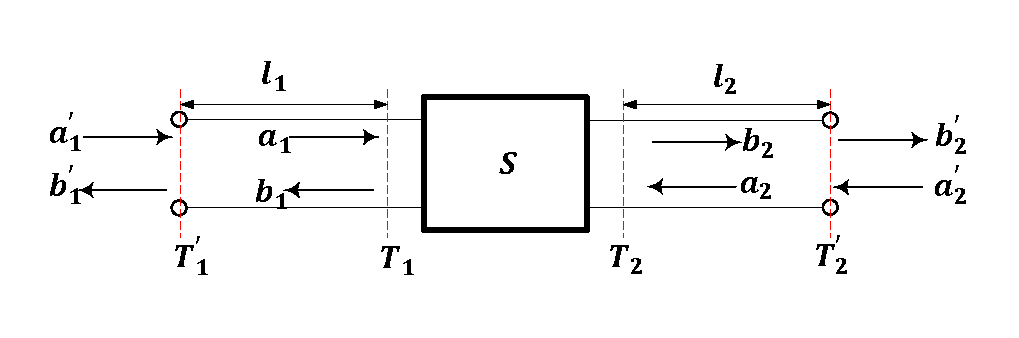
\includegraphics[width=10cm]{Cha5//fig5-18.pdf}
              \end{figure}
              \begin{gather*}
                  [S]=\begin{bmatrix*}
                      S_{11} & S_{12} \\
                      S_{21} & S_{22} \\
                  \end{bmatrix*}
              \end{gather*}
    \end{enumerate}
\end{frame}

\begin{frame}{微波网络参量}
    \begin{enumerate}
        \resume
        \item 参考面移动对网络参数的影响\\
              $a^{'}$超前于$a$,而$b^{'}$滞后于$b$
              \begin{align*}
                   & \begin{bmatrix*}
                         a_1^{'} \\
                         a_2^{'} \\
                     \end{bmatrix*}
                  =
                  \begin{bmatrix*}
                      \mathrm{e}^{\mathrm{j}\theta_1} & 0 \\
                      0 & \mathrm{e}^{\mathrm{j}\theta_2} \\
                  \end{bmatrix*}
                  \begin{bmatrix*}
                      a_1 \\
                      a_2 \\
                  \end{bmatrix*}
                  \qquad
                  \begin{bmatrix*}
                      b_1^{'} \\
                      b_2^{'} \\
                  \end{bmatrix*}
                  =
                  \begin{bmatrix*}
                      \mathrm{e}^{-\mathrm{j}\theta_1} & 0 \\
                      0 & \mathrm{e}^{-\mathrm{j}\theta_2} \\
                  \end{bmatrix*}
                  \begin{bmatrix*}
                      b_1 \\
                      b_2 \\
                  \end{bmatrix*}            \\
                   & \begin{cases}
                         \theta_1=\beta\cdot l_1 \\
                         \theta_2=\beta\cdot l_2
                     \end{cases}
              \end{align*}
    \end{enumerate}
\end{frame}

\begin{frame}{微波网络参量}
    \begin{enumerate}
        \resume
        \item 参考面移动对网络参数的影响\\
              \begin{align*}
                   & \begin{bmatrix*}
                         b_1^{'} \\
                         b_2^{'} \\
                     \end{bmatrix*}
                  =
                  \begin{bmatrix*}
                      \mathrm{e}^{-\mathrm{j}\theta_1} & 0 \\
                      0 & \mathrm{e}^{-\mathrm{j}\theta_2} \\
                  \end{bmatrix*}
                  \begin{bmatrix*}
                      b_1 \\
                      b_2 \\
                  \end{bmatrix*}
                  \qquad
                  \begin{bmatrix*}
                      b_1 \\
                      b_2 \\
                  \end{bmatrix*}
                  =
                  \begin{bmatrix*}
                      S_{11} & S_{12} \\
                      S_{21} & S_{22} \\
                  \end{bmatrix*}
                  \begin{bmatrix*}
                      a_1 \\
                      a_2 \\
                  \end{bmatrix*}    \\
                  \rightarrow
                   & \begin{bmatrix*}
                         b_1^{'} \\
                         b_2^{'} \\
                     \end{bmatrix*}
                  =
                  \begin{bmatrix*}
                      \mathrm{e}^{-\mathrm{j}\theta_1} & 0 \\
                      0 & \mathrm{e}^{-\mathrm{j}\theta_2} \\
                  \end{bmatrix*}
                  \begin{bmatrix*}
                      S_{11} & S_{12} \\
                      S_{21} & S_{22} \\
                  \end{bmatrix*}
                  \begin{bmatrix*}
                      a_1 \\
                      a_2 \\
                  \end{bmatrix*}
                  \qquad
                  \begin{bmatrix*}
                      a_1^{'} \\
                      a_2^{'} \\
                  \end{bmatrix*}
                  =
                  \begin{bmatrix*}
                      \mathrm{e}^{\mathrm{j}\theta_1} & 0 \\
                      0 & \mathrm{e}^{\mathrm{j}\theta_2} \\
                  \end{bmatrix*}
                  \begin{bmatrix*}
                      a_1 \\
                      a_2 \\
                  \end{bmatrix*}    \\
                  \rightarrow
                   & \begin{bmatrix*}
                         b_1^{'} \\
                         b_2^{'} \\
                     \end{bmatrix*}
                  =
                  \begin{bmatrix*}
                      \mathrm{e}^{-\mathrm{j}\theta_1} & 0 \\
                      0 & \mathrm{e}^{-\mathrm{j}\theta_2} \\
                  \end{bmatrix*}
                  \begin{bmatrix*}
                      S_{11} & S_{12} \\
                      S_{21} & S_{22} \\
                  \end{bmatrix*}
                  \begin{bmatrix*}
                      \mathrm{e}^{\mathrm{j}\theta_1} & 0 \\
                      0 & \mathrm{e}^{\mathrm{j}\theta_2} \\
                  \end{bmatrix*}^{-1}
                  \begin{bmatrix*}
                      a_1^{'} \\
                      a_2^{'} \\
                  \end{bmatrix*}
              \end{align*}
              \begin{align*}
                  \begin{bmatrix*}
                      b_1^{'} \\
                      b_2^{'} \\
                  \end{bmatrix*}
                  =
                  \begin{bmatrix*}
                      S_{11}^{'} & S_{12}^{'} \\
                      S_{21}^{'} & S_{22}^{'} \\
                  \end{bmatrix*}
                  =
                  \begin{bmatrix*}
                      S_{11}\cdot\mathrm{e}^{-\mathrm{j}2\theta_1} & S_{12}\cdot\mathrm{e}^{-\mathrm{j}(\theta_1+\theta_2)} \\
                      S_{21}\cdot\mathrm{e}^{-\mathrm{j}(\theta_1+\theta_2)} & S_{22}\cdot \mathrm{e}^{-\mathrm{j}2\theta_2} \\
                  \end{bmatrix*}
                  \begin{bmatrix*}
                      a_1^{'} \\
                      a_2^{'} \\
                  \end{bmatrix*}
              \end{align*}
    \end{enumerate}
\end{frame}

\begin{frame}{微波网络参量}
    \begin{enumerate}
        \resume
        \item 参考面移动对网络参数的影响
              \begin{align*}
                  \begin{bmatrix*}
                      b_1^{'} \\
                      b_2^{'} \\
                  \end{bmatrix*}
                  =
                  \begin{bmatrix*}
                      S_{11}\cdot\mathrm{e}^{-\mathrm{j}2\theta_1} & S_{12}\cdot\mathrm{e}^{-\mathrm{j}(\theta_1+\theta_2)} \\
                      S_{21}\cdot\mathrm{e}^{-\mathrm{j}(\theta_1+\theta_2)} & S_{22}\cdot \mathrm{e}^{-\mathrm{j}2\theta_2} \\
                  \end{bmatrix*}
                  \begin{bmatrix*}
                      a_1^{'} \\
                      a_2^{'} \\
                  \end{bmatrix*}
                  =[S^{'}]
                  \begin{bmatrix*}
                      a_1^{'} \\
                      a_2^{'} \\
                  \end{bmatrix*}
              \end{align*}
              \begin{itemize}
                  \item 结论:参考面的移动,仅对$[S]$的相位产生影响
              \end{itemize}
              \begin{gather*}
                  \begin{bmatrix*}
                      S^{'}
                  \end{bmatrix*}
                  =
                  \begin{bmatrix*}
                      \mathrm{e}^{-\mathrm{j}\theta_1} & 0 \\
                      0 & \mathrm{e}^{-\mathrm{j}\theta_2} \\
                  \end{bmatrix*}
                  \begin{bmatrix*}
                      S_{11} & S_{12} \\
                      S_{21} & S_{22} \\
                  \end{bmatrix*}
                  \begin{bmatrix*}
                      \mathrm{e}^{-\mathrm{j}\theta_1} & 0 \\
                      0 & \mathrm{e}^{-\mathrm{j}\theta_2} \\
                  \end{bmatrix*}\\
                  \begin{bmatrix*}
                      S^{'}
                  \end{bmatrix*}
                  =
                  \begin{bmatrix*}
                      P
                  \end{bmatrix*}
                  \begin{bmatrix*}
                      S
                  \end{bmatrix*}
                  \begin{bmatrix*}
                      P
                  \end{bmatrix*}\\
                  \begin{bmatrix*}
                      P
                  \end{bmatrix*}
                  =
                  \begin{cases}
                      \mathrm{e}^{-\mathrm{j}\theta} \quad \text{参考面向外移动} \\
                      \mathrm{e}^{\mathrm{j}\theta} \quad \text{参考面向内移动}
                  \end{cases}
              \end{gather*}
    \end{enumerate}
\end{frame}

\begin{frame}{微波网络参量}
    \begin{table}
        \caption{基本电路单元的网络参量矩阵}
        \tiny % 设置表格内字体大小
        \renewcommand\arraystretch{1.25} % 设置行宽为初始值1.25倍
        \begin{tabular}{|c|c|c|c|}
            \hline
            电路
             & \begin{minipage}[b]{0.25\columnwidth}
                   \centering
                   \raisebox{-.5\height}{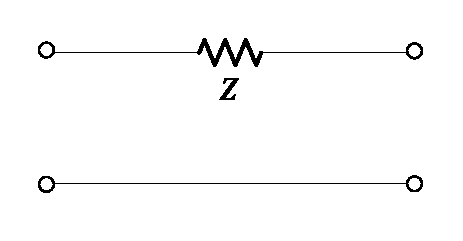
\includegraphics[width=2.5cm]{Cha5//fig5-20.pdf}}
               \end{minipage}
             & \begin{minipage}[b]{0.25\columnwidth}
                   \centering
                   \raisebox{-.5\height}{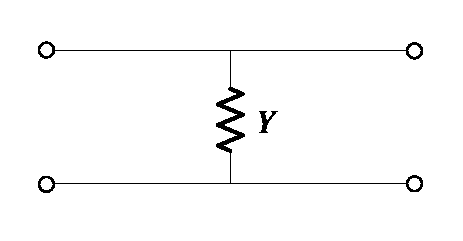
\includegraphics[width=2.5cm]{Cha5//fig5-19.pdf}}
               \end{minipage}
             & \begin{minipage}[b]{0.25\columnwidth}
                   \centering
                   \raisebox{-.5\height}{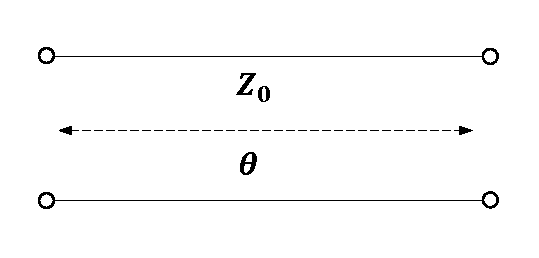
\includegraphics[width=2.5cm]{Cha5//fig5-17.pdf}}
               \end{minipage}                              \\
            \hline
            $[Z]$
             &
             & $   \begin{bmatrix*}
                           \frac{1}{y} & \frac{1}{y} \\
                           \frac{1}{y} & \frac{1}{y} \\
                       \end{bmatrix*}$
             & $   \begin{bmatrix*}
                           -\mathrm{j}Z_0\cot\theta & -\mathrm{j}Z_0\csc\theta \\
                           -\mathrm{j}Z_0\csc\theta & -\mathrm{j}Z_0\cot\theta \\
                       \end{bmatrix*}$                    \\
            \hline
            $[Y]$
             & $ \begin{bmatrix*}
                         \frac{1}{z} & -\frac{1}{z} \\
                         -\frac{1}{z} & \frac{1}{z} \\
                     \end{bmatrix*}$
             &
             & $   \begin{bmatrix*}
                           -\mathrm{j}\frac{1}{Z_0}\cot\theta & \mathrm{j}\frac{1}{Z_0}\csc\theta \\
                           \mathrm{j}\frac{1}{Z_0}\csc\theta & -\mathrm{j}\frac{1}{Z_0}\cot\theta \\
                       \end{bmatrix*}$ \\
            \hline
            $[A]$
             & $ \begin{bmatrix*}
                         1 & z \\
                         0 & 1 \\
                     \end{bmatrix*}$
             & $ \begin{bmatrix*}
                         1 & 0 \\
                         y & 1 \\
                     \end{bmatrix*}$
             & $ \begin{bmatrix*}
                         \cos\theta & \mathrm{j}Z_0\sin\theta \\
                         \mathrm{j}\frac{1}{Z_0}\sin\theta & \cos\theta \\
                     \end{bmatrix*}$                           \\
            \hline
            $[S]$
             & $ \begin{bmatrix*}
                         \frac{z}{2+z} & \frac{2}{2+z} \\
                         \frac{2}{2+z} & \frac{z}{2+z} \\
                     \end{bmatrix*}$
             & $ \begin{bmatrix*}
                         \frac{-y}{2+y} & \frac{2}{2+y} \\
                         \frac{2}{2+y} & \frac{-y}{2+y} \\
                     \end{bmatrix*}$
             & $ \begin{bmatrix*}
                         0 & \mathrm{e}^{\mathrm{j}\theta} \\
                         \mathrm{e}^{\mathrm{j}\theta} & 0 \\
                     \end{bmatrix*}$                                        \\
            \hline
        \end{tabular}
    \end{table}
\end{frame}

\subsection{微波网络参量的性质}
\begin{frame}{微波网络参量的性质}
    \begin{enumerate}
        \item 互易性\\
              \begin{itemize}
                  \item 当无源二端口网络中填充各向同性媒质时,该网络为互易网络,此时网络参量应满足互易条件。互易网络的阻抗和导纳矩阵是对称的。
              \end{itemize}
              \begin{gather*}
                  [Z]^T=[Z],Z_{kj}=Z_{jk}(j\neq k)\\
                  [Y]^T=[Y],Y_{kj}=Y_{jk}(j\neq k)\\
                  [S]^T=[S],S_{kj}=S_{jk}(j\neq k)
              \end{gather*}
              \saveenum
    \end{enumerate}
\end{frame}

\begin{frame}{微波网络参量的性质}
    \begin{enumerate}
        \item 互易性 \\
              证明:
              \begin{align*}
                  [z][i]=[z][a]-[z][b]=[v]=[a]+[b] \\
                  ([z]+[I])[b]=([z]-[I])[a]        \\
                  \Rightarrow[S]=([z]+[I])^{-1}([z]-[I])
              \end{align*}
              再根据
              \begin{align*}
                  \begin{cases}
                      [a]=\frac{1}{2}([v]+[i])=\frac{1}{2}([z]+[I])[i] \\
                      [b]=\frac{1}{2}([v]-[i])=\frac{1}{2}([z]-[I])[i]
                  \end{cases} \\
                  \Rightarrow [S]=([z]-[I])([z]+[I])^{-1}          \\
                  \Rightarrow [S]^T=([z]+[I])^{-1}([z]-[I])
              \end{align*}
    \end{enumerate}
\end{frame}

\begin{frame}{微波网络参量的性质}
    \begin{enumerate}
        \resume
        \item 对称性
              \begin{itemize}
                  \item 对称网络可以反向使用,性能不变
                  \item $Z_{11}=Z_{22},Z_{12}=Z_{21}$
                  \item $Y_{11}=Y_{22},Y_{12}=Y_{21}$
                  \item $S_{11}=S_{22},S_{12}=S_{21}$
                  \item 对称网络首先必须是互易网络
              \end{itemize}
              \saveenum
    \end{enumerate}
\end{frame}

\begin{frame}{微波网络参量的性质}
    \begin{enumerate}
        \resume
        \item 无耗网络$S$参量的幺正性\\
              对于无耗网络,因其损耗功率$P=0$,则
              \begin{gather*}
                  [I]-[S]^\dagger[S]=0
              \end{gather*}
              \begin{itemize}
                  \item $[\quad]^\dagger$ —— Hermite符号,表示共轭转置或转置共轭\\
                        \begin{align*}
                            [\quad]^\dagger=([\quad]^{*})^T=([\quad]^T)^{*}
                        \end{align*}
              \end{itemize}
    \end{enumerate}
\end{frame}

\begin{frame}{微波网络参量的性质}
    \begin{enumerate}
        \resume
        \item 无耗网络$S$参量的幺正性
              \begin{align*}
                  p & =\frac{1}{2}\mathrm{Re}(vi^*)=\frac{1}{2}\mathrm{Re}[(a+b)(a^*-b^*)] \\
                    & =\frac{1}{2}(aa^*-bb^*)+\frac{1}{2}\mathrm{Re}(a^*b-ab^*)
              \end{align*}
              后一项的实部显然等于$0$,于是有
              \begin{align*}
                   & p=\frac{1}{2}(aa^*-bb^*)                                               \\
                   & p^+=\frac{1}{2}\lvert a\rvert^2 \qquad p^-=\frac{1}{2}\lvert b\rvert^2 \\
                   & p=p^+-p^-=\frac{1}{2}(\lvert a\rvert^2-\lvert b\rvert^2)
              \end{align*}
              物理意义:端口功率等于入射功率减去散射功率。
    \end{enumerate}
\end{frame}

\begin{frame}{微波网络参量的性质}
    \begin{enumerate}
        \resume
        \item 无耗网络$S$参量的幺正性\\
              无耗条件为
              $$p=0,或者aa^*-bb^*=0$$
              假如对于双端口网络,有
              \begin{align*}
                  a_1a_1^*+a_2a_2^*=
                  \begin{bmatrix*}
                      a_1^*,a_2^*
                  \end{bmatrix*}
                  \begin{bmatrix*}
                      a_1 \\
                      a_2 \\
                  \end{bmatrix*}
                  =
                  \begin{bmatrix*}
                      a
                  \end{bmatrix*}^\dagger
                  \begin{bmatrix*}
                      a
                  \end{bmatrix*}
              \end{align*}
              于是,把多口网络的无耗条件写成
              \begin{align*}
                   & \begin{bmatrix*}
                         a
                     \end{bmatrix*}^\dagger
                  \begin{bmatrix*}
                      a
                  \end{bmatrix*}
                  -
                  \begin{bmatrix*}
                      b
                  \end{bmatrix*}^\dagger
                  \begin{bmatrix*}
                      b
                  \end{bmatrix*}
                  =0                        \\
                   & \begin{bmatrix*}
                         a
                     \end{bmatrix*}^\dagger
                  \begin{bmatrix*}
                      a
                  \end{bmatrix*}
                  -
                  \begin{bmatrix*}
                      a
                  \end{bmatrix*}^\dagger
                  \begin{bmatrix*}
                      S
                  \end{bmatrix*}^\dagger
                  \begin{bmatrix*}
                      S
                  \end{bmatrix*}
                  \begin{bmatrix*}
                      a
                  \end{bmatrix*}
                  =0
              \end{align*}
              即
              \begin{gather*}
                  \begin{bmatrix*}
                      a
                  \end{bmatrix*}^\dagger
                  \left\{
                  \begin{bmatrix*}
                      I
                  \end{bmatrix*}
                  -
                  \begin{bmatrix*}
                      S
                  \end{bmatrix*}^\dagger
                  \begin{bmatrix*}
                      S
                  \end{bmatrix*}
                  \right\}
                  \begin{bmatrix*}
                      a
                  \end{bmatrix*}
                  =0
              \end{gather*}
    \end{enumerate}
\end{frame}

\begin{frame}{微波网络参量的性质}
    \begin{enumerate}
        \resume
        \item 无耗网络$S$参量的幺正性\\
              考虑$[a]$激励的任意性,可知
              \begin{align*}
                  \begin{bmatrix*}
                      I
                  \end{bmatrix*}
                  -
                  \begin{bmatrix*}
                      S
                  \end{bmatrix*}^\dagger
                  \begin{bmatrix*}
                      S
                  \end{bmatrix*}
                  =0
              \end{align*}
              当网络\textbf{互易无耗}时,即
              \begin{gather*}
                  [S]^T=[S] \rightarrow [S]^\dagger=[S]^*\\
                  [S]^\dagger [S]=[S]^*[S]=[I]\\
                  \sum_{k=1}^N S_{ki}S_{kj}^*=\delta_{ij} \qquad 对于所有的 i,j\\
              \end{gather*}
    \end{enumerate}
\end{frame}

\begin{frame}
    \begin{enumerate}
        \resume
        \item 无耗网络$S$参量的幺正性
              \begin{align*}
                  \begin{matrix*}
                      \sum\limits_{k=1}^N S_{ki}S_{ki}^*=1 & i=j & \text{\scriptsize{无耗网络S参量的单元特性}} \\
                      &     & \text{\scriptsize{说明[S]的任一列与此列的共轭点乘等于1}} \\
                      \sum\limits_{k=1}^N S_{ki}S_{kj}^*=0 & i\neq j & \text{\scriptsize{无耗网络S参量的零特性}} \\
                      &     & \text{\scriptsize{说明[S]的任一列与不同列的共轭点乘为0}}\\
                  \end{matrix*}
              \end{align*}
              若网络是\textbf{互易}的,则$[S]$是对称的,对于散射参量的各行,可以有同样的特征。
    \end{enumerate}
\end{frame}

\subsection{二端口微波网络的工作特性参量}
\begin{frame}{二端口微波网络的工作特性参量}
    \begin{enumerate}
        \item 电压传输系数$T$
              \begin{itemize}
                  \item 网络输出端接匹配负载时,输出端参考面上的反射波电压与入射参考面上的入射波电压之比。
              \end{itemize}
              \begin{figure}
                  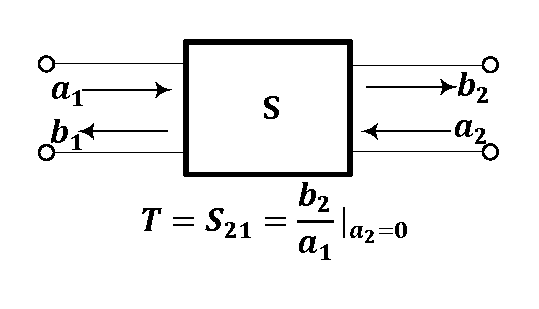
\includegraphics[width=7cm]{Cha5//fig5-21.pdf}
              \end{figure}
              \saveenum
    \end{enumerate}
\end{frame}

\begin{frame}{二端口微波网络的工作特性参量}
    \begin{enumerate}
        \resume
        \item 插入衰减$L_i$
              \begin{itemize}
                  \item 网络未插入前负载吸收的功率与网络插入后负载吸收的功率之比的分贝数。
              \end{itemize}
              \begin{figure}
                  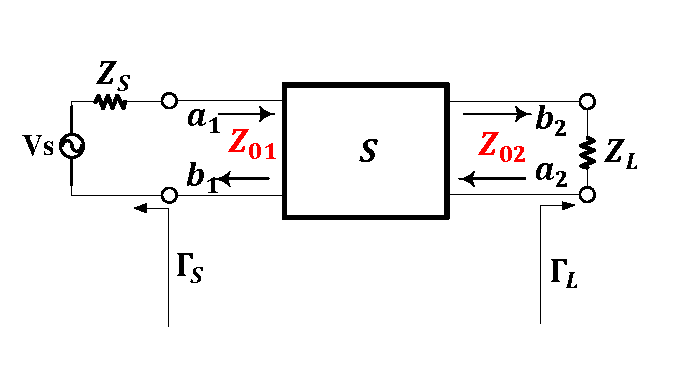
\includegraphics[width=7cm]{Cha5//fig5-22.pdf}
              \end{figure}
              未插入前负载的吸收功率:
              $$P_{L0}=\frac{1}{2}\lvert a_1\rvert^2\left(1-\lvert\Gamma_L\rvert^2\right)$$
              网络插入后负载的吸收功率
              \begin{align*}
                  P_L=\frac{1}{2}\lvert b_2\rvert^2\left(1-\lvert\Gamma_L\rvert^2\right)
              \end{align*}
    \end{enumerate}
\end{frame}

\begin{frame}{二端口微波网络的工作特性参量}
    \begin{enumerate}
        \resume
        \item 插入衰减$L_i$
              \begin{align*}
                  P_L & =\frac{1}{2}\lvert b_2\rvert^2\left(1-\lvert\Gamma_L\rvert^2\right)\qquad b_2=\frac{S_{21}a_1}{1-S_{22}\Gamma_L}  \\
                      & =\frac{1}{2}\frac{\lvert S_{21}a_1\rvert^2\left(1-\lvert\Gamma_L\rvert^2\right)}{\lvert 1-S_{22}\Gamma_L\rvert^2}
              \end{align*}
              $$L_i=10\lg\frac{P_{L0}}{P_L}=10\lg\frac{\lvert 1-S_{22}\Gamma_L\rvert^2}{\lvert S_{21}\rvert^2}$$
              \saveenum
    \end{enumerate}
\end{frame}

\begin{frame}{二端口微波网络的工作特性参量}
    \begin{enumerate}
        \resume
        \item 工作衰减$L_A$
              \begin{itemize}
                  \item 网络输入输出端接匹配负载时,则插入衰减仅与网络参量有关,称为工作衰减$L_A$
              \end{itemize}
              $$L_A=10\lg\frac{1}{\lvert S_{21}\rvert^2} \quad dB$$
              \begin{itemize}
                  \item 无耗网络
              \end{itemize}
              $$L_A=10\lg\frac{1}{1-\lvert S_{11}\rvert^2} \quad dB$$
              \begin{align*}
                  L_A&=10\lg\left(\frac{1}{1-\lvert S_{11}\rvert^2}\cdot\frac{1-\lvert S_{11}\rvert^2}{\lvert S_{21}\rvert^2}\right)\\
                     &=
                  \begin{matrix*}
                      10\lg\left(\frac{1}{1-\lvert S_{11}\rvert^2}\right) & + & 10\lg\left(\frac{1-\lvert S_{11}\rvert^2}{\lvert S_{21}\rvert^2}\right)\\
                      \text{\scriptsize{反射衰减}} & & \text{\scriptsize{吸收衰减}}\\
                  \end{matrix*}
              \end{align*}
              \saveenum
    \end{enumerate}
\end{frame}

\begin{frame}{二端口微波网络的工作特性参量}
    \begin{enumerate}
        \resume
        \item 插入相移$\theta$
              \begin{itemize}
                  \item 网络输出端接匹配负载时,输出端反射波对输入端入射波的相移。即为$b_2$与$a_1$的相位差
                        \begin{itemize}
                            \item 令输入端入射波电压和输出端反射波电压分别为
                        \end{itemize}
              \end{itemize}
              \begin{gather*}
                  a_1=\lvert a_1\rvert\mathrm{e}^{\mathrm{j}\varphi_1} \qquad b_2=\lvert b_2\rvert\mathrm{e}^{\mathrm{j}\varphi_2}\\
                  T=\frac{b_2}{a_1}\bigg|_{a_2=0}=\lvert S_{21}\rvert\mathrm{e}^{\mathrm{j}(\varphi_2-\varphi_1)} \\
                  \theta=\mathrm{arg}T=\mathrm{arg}S_{21}
              \end{gather*}
        \item 插入驻波比$\rho$
              \begin{itemize}
                  \item 网络输出端接匹配负载时,输入端的驻波比
                        \begin{itemize}
                            \item 输入端驻波比与输入端反射系数模的关系为
                        \end{itemize}
              \end{itemize}
              $$\rho=\frac{1+|\Gamma|}{1-|\Gamma|} \quad \rho=\frac{1+|S_{11}|}{1-|S_{11}|}$$
    \end{enumerate}
\end{frame}

\subsection{微波网络的组合}
\begin{frame}{微波网络的组合}

\end{frame}

\subsection{二端口网络的等效电路}
\begin{frame}{二端口网络的等效电路}

\end{frame}

\subsection{信号流图分析及其应用}
\begin{frame}{信号流图分析及其应用}

\end{frame}

